\documentclass[11pt]{article}
\usepackage[margin=1in]{geometry}
\usepackage{graphicx}
\usepackage{subcaption}
\usepackage{url}
\usepackage{dirtree}
\usepackage{hyperref}
\usepackage{longtable}
\usepackage{bbm}
\usepackage{amsfonts}
\usepackage{amsfonts}

\usepackage{glossaries}

\makeglossaries{}

\newglossaryentry{CI/CD}{
  name={CI/CD},
  description={Continuous Integration and Continuous Development. The process of
  automating software testing, building, and deployment.}
}

\newglossaryentry{CLI}
{
    name={CLI},
    description={A command-line interface (CLI) is a text-based user interface (UI) used to run programs, manage computer files and interact with the computer.}
}

\newglossaryentry{DSL}
{
    name=DSL,
    description={A computer language that is specialized to a particular application/domain}
}

\newglossaryentry{target execution}
{
    name=target execution,
    description={An instance of a \gls{target} that needs to be completed as per described in the project definition}
}

\newglossaryentry{cache}
{
    name=cache,
    description={to save something to computers memory or local storage. An example would be the output of a \gls{target execution}}
}

\newglossaryentry{project definition}
{
    name=project definition,
    description={A file containing information pertaining a project, an example could be the language that was used}
}

\newglossaryentry{metadata}
{
    name=metadata,
    description={any custom data that the project owner wants to add about the project}
}

\newglossaryentry{target}
{
    name=target,
    description={An execution target, a recipe or command for what you want to do to/with the project, ie build and deploy the project, run tests, ect}
}

\newglossaryentry{monorepo}
{
  name=monorepo,
  description={A software-development strategy in which the code for a number of projects is stored in the same repository.}
}

\title{\textbf{4ZP6 Project - Deliverable 7}}
\author{Usman Asad --- asadu  --- 400199934\\
  Ali Khan --- khana238  --- 400211680\\
  Omar Alkersh --- alkersho --- 400214491 \\
  Ahmed Al-sabounchi --- alsaboaa --- 001327403 \\
  Tanveer Shakeel --- shakeelt --- 400226915}

\begin{document}

\maketitle
\tableofcontents
\newpage

\section{Introduction}
Gitlab URL: https://gitlab.cas.mcmaster.ca/alsaboaa/monorepo \\
\\
Submission commit hash: 6dea39
\subsection{Purpose}

This document is intended to be read by programmers, it contains the projects design
decisions pertaining to the software architecture, language, application format,
and internal module API. The focus of the documentation is to provide guidance on the
processes of the program, a high level overview of how it's actions are executed. It
also provides some guidance on the internal code organization. The latter is subject
to change depending on practical findings and use case.

\subsection{Scope}

This project is a compiled \Gls{CLI} tool used to manage \glspl{monorepo}. This
tool should allow the user to check for changes in the code, execute \glspl{target},
check project dependencies, and provide tooling to aid in \Gls{CI/CD} pipelines
where appropriate.
\\\\
The goal is to provide a portable, fast, and easy to use program to help in
CI/CD pipelines for \glspl{monorepo}.

\subsection{Overview}

This document consists of design decisions, module designs, and diagrams
clarifying the design of the project. Any part of this document is subject to
change based on need and experimentation.
\\\\
The decision mainly consists of the language choice and the architecture. The
module design is meant to clarify the module breakdown, the API of each module,
and the module interactions and dependencies. The
\hyperref[sec:diagrams]{Diagrams} section provides more insight on the operation
of the program and how different modules interact with each other. The diagram
section is more concrete compared to the other sections and is not as likely
to change.
\\\\
For the module specifications, the sub items in the exported types represent
state variables.

\subsection{Definitions}

\printglossary[title=\normalsize\vspace*{-1.5\baselineskip}, toctitle=]
\section{System Overview}

The program is a \Gls{CLI} tool to manage \glspl{monorepo} and aid in
\gls{CI/CD} operations. It is meant to be light weight \& portable, and has no
trivial dependencies. The tool provides the abilities to run \glspl{target}
concurrently, define dependencies on the project level, and on the operation
level. It should also be able to perform operations on the projects; including
but not limited to creating, searching, and listing.
\\\\
A number of companies use the \gls{monorepo} development philosophy, and more
are adopting it. Without considering in-house solutions, there is currently only
one real competitor in this space with others catching up. \Glspl{monorepo} are
more complicated to manage than traditional repositories, greatly benefiting
from a tool to help automate and manage them.
\\\\
There other \gls{monorepo} tools in the space such
as; \href{https://nx.dev/}{NX}, \href{https://bazel.build/}{Bazel}, and others.
All of them have features that the others lack, or are slow to run or slow to
load in \gls{CI/CD} environments (NX is a node application).
\\\\
This program is aimed to combine their strengths, and best features based on our
experience with them. It is meant to fill a gap that none of these programs fill.

\section{System Architecture}

\subsection{Architectural Design}

We have opted for a ``component'' based architecture. The different features and
logic are encapsulated in different components and modules as described in the
\hyperref[sec:modules]{Modules} section.
\\\\
%% Talk about the different modules and the functions that they need to fulfill
The modules and their definitions are subject to change.
\\\\
There are 5 modules; command runner, parser, data, algorithms, and common
utility. In the final product, these modules were implemented in the /src/pkg/ folder, with the names of the files corresponding to the modules that were implemented within them. The command runner module can be found in /src/pkg/commands/run.go.

\begin{itemize}
\item The command runner is responsible for running the correct command
  depending on the user's input. It also provides any specialized data definitions.

\item The parser provides functions to parse files to their respective data types.

\item The data modules provides the data definitions for the program. Mainly the
  \gls{project definition} and workspace definitions.

\item The algorithms module provides functions and data types to schedule the
  execution of \gls{target} and tasks.

\item The common utilities module is mainly a workaround to Golang's import
  limitation. It doesn't allow cyclic imports. This module should contain all
  the common functionality to avoid cyclic imports.
\end{itemize}

\subsection{Design Rationale}
\subsubsection{Language}
\label{sec:lang}

The language that we decided to write the program in is Go. We needed a compiled
and type checked language. We decided to choose Go over C/C++ and Java due to usability and
safety concerns. C/C++ have the memory issues that needs to be addressed and managed; and
Java is disliked and slow. Furthermore, it requires a JVM to be installed, which
defeats the purpose of small installation size.
\\\\
We also considered Rust, but decided against it due to the learning curve and
the majority of the team not having experience with it.

\subsubsection{Software Architecture}

We decided on a component based design. This should allow us to expand the
software without significant rewrites when we want to extend its functionality.
In addition, it allows us to work on separate parts in parallel accelerating
development.
\\\\
Most other software architectures, client-server or MVC, are not relevant to
this project nor do they provide any benefit. This program consists only of a
compiled CLI program, no external communication is required in this iteration.

\subsection{Decomposition}

The following diagram mainly concerns itself with the ``import'' relation that
the components have, which component imports which component. There is no
inheritance or extension relation. All the data types are defined once and not
extended beyond their definition.

\newpage
\subsubsection{Diagrams}

\begin{figure}[h!]
  \centering
  \begin{subfigure}{0.5\linewidth}
    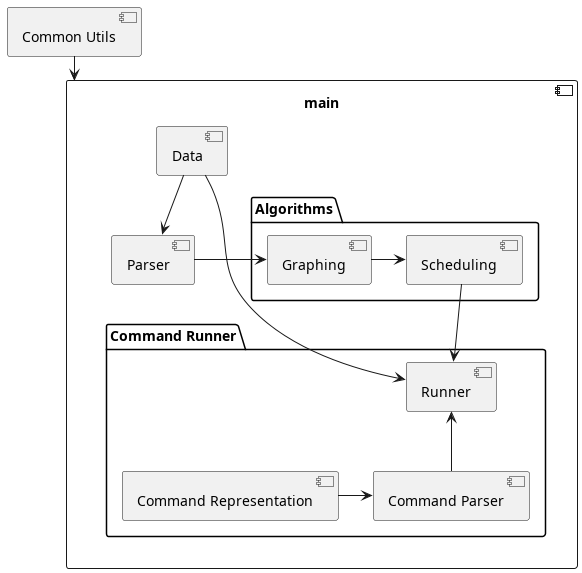
\includegraphics[width=\linewidth]{diags/components.png}
    \caption{\label{fig:comp}Component Diagram}
  \end{subfigure}
  \begin{subfigure}{0.15\linewidth}
    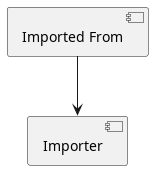
\includegraphics[width=\linewidth]{diags/comp_legend.png}
    \caption{\label{fig:comp}Legend}
  \end{subfigure}
  \caption{Component Composition Diagram}
\end{figure}

\begin{figure}[h!]
\end{figure}

\begin{figure}[h!]
  \centering
  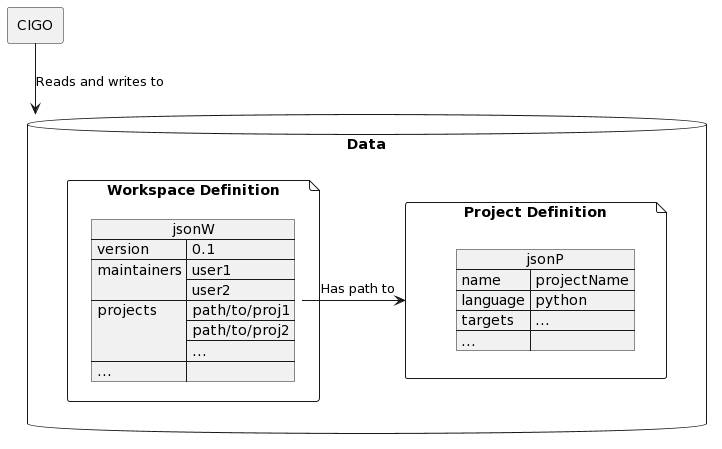
\includegraphics[width=0.8\linewidth]{diags/system.png}
  \caption{Data Interaction and store}
  \label{fig:storage}
\end{figure}

Note that the data can be stored as a JSON, YAML, or a DSL that is yet to be
developed. See figure \ref{fig:storage}.


\newpage
\section{Modules}
\label{sec:modules}

Each module represents a package. One module may export multiple types and
define functions over many types. No function is assumed to be a ``class method''
unless specified.

\subsection{Command Runner}
\label{mod:command}

\subsubsection{Exported Types}

The exported types are representations of the possible command line arguments
that the program accepts. They are used to parse them and represent them in
code. The sub items are struct fields, which represent options or the command.

\begin{itemize}
\item $Args$:
  \begin{itemize}
  \item help: $Boolean$
  \item dry run: $Boolean$
  \item version: $Boolean$
  \item command: $Command$
  \end{itemize}
\item $Command$ --- enum:
  \begin{itemize}
  \item $List$
  \item $Search$:
    \begin{itemize}
    \item searchItems: $map[key]value$

    \item limit: $\mathbbm{N}$
    \end{itemize}
  \item $Run$:
    \begin{itemize}
    \item project: $string | seq(string)$
    \item target: $string$
    \end{itemize}
  \item $GetChanges$:
    \begin{itemize}
    \item baseRef: $string$
    \item targetRef: $string | null$
    \end{itemize}
  \end{itemize}
\end{itemize}

\subsubsection{Functions}

\begin{tabular}[h!]{l|l|l|p{6cm}}
  \textbf{Name} & \textbf{Input} & \textbf{Output} & \textbf{Description} \\
  \hline
  parse & string & Args & Parses the command arguments to an $Args$ type.\\
  \hline
  run & Args & $\mathbbm{Z}$ & Runs the given command based on the data within. Returns the command success code.
\end{tabular}

\vspace{2em}

\textbf{Definitions}\\

$parse(string):$
\begin{itemize}
\item transition:
  \begin{itemize}
  \item $help :=$ The help flag is present.
  \item $dryRun :=$ The dry run flag is present.
  \item $version :=$ The version flag is present.

  \item $command :=$ The sub command to execute.
  \end{itemize}
\item output: $out := Self$
\item exception: $exc :=$ Parse failure.
\end{itemize}

\vspace{1em}
$run(args):$
\begin{itemize}
\item output: $out :=$ The command status code. Non-zero if the command failed.
\item exceptions: None
\end{itemize}

\subsection{Parser}
\label{mod:parser}
This module contains code for reading project definitions and workspace/repo files
in .yaml, .json or from our Domain Specific Language
\subsubsection{Uses/Imports}
\begin{itemize}
  \item Data Module
  \item External JSON library
\end{itemize}

\subsubsection{Exported Types}
\begin{itemize}
  \item Parser = ?
  \item FileType = {JSON}
\end{itemize}

\subsubsection{Functions}
\begin{longtable}{l|l|l|l}
  \textbf{Name} & \textbf{Inputs} & \textbf{Output} & \textbf{Description} \\ \hline
  decodeProjectDef &
    String, FileType &
    ProjectDefinition &
    \begin{tabular}[c]{@{}l@{}}Takes in a filePath, and a file type,\\decodes the file and returns an\\instance of a ProjectDefinition struct\end{tabular} \\\hline
  encodeProjectDef &
  \begin{tabular}[c]{@{}l@{}}ProjectDefinition, \\ string, \\ FileType\end{tabular} &
    Encoded String &
    \begin{tabular}[c]{@{}l@{}}Takes in a ProjectDefinition, a file path,\\and a FileType and writes\\the deserialized content to the file.\end{tabular} \\\hline
  decodeWorkspace &
    String, FileType &
    Workspace &
    \begin{tabular}[c]{@{}l@{}}Takes in a filePath, and a file type,\\decodes the file and returns an\\instance of a Workspace struct\end{tabular} \\\hline
  encodeWorkspace &
    \begin{tabular}[c]{@{}l@{}}Workspace, \\String, \\ FileType\end{tabular} &
    Encoded String &
    \begin{tabular}[c]{@{}l@{}}Takes in a Workspace, a file path,\\and a FileType and writes the\\deserialized content to the file.\end{tabular}
  \end{longtable}

  \vspace{2em}
  \textbf{Definitions}\\

  $decodeProjectDef(content, type):$
  \begin{itemize}
  \item output: $out :=$ The serialized ProjectDefinition.
  \item exception: $exc :=$
    \begin{align*}
      \text{ file doesn't exist } &\implies FileNotFound|\\
      \text{ serialization error } &\implies InvalidFormat|\\
      True &\implies none
    \end{align*}
  \end{itemize}

  \vspace{1em}
  $encodeProjectDef(def, path, type):$
  \begin{itemize}
  \item output: $out :=$ Write to the file the deserialized project definition.
  \item exception: $exc :=$
    \begin{align*}
      \text{ Failed to write } &\implies IOError|\\
      \text{ Bad path } &\implies IllegalPath|\\
      \text{ deserialization error } &\implies EncodingErr|\\
      True &\implies none
    \end{align*}
  \end{itemize}
  \vspace{1em}
  $decodeWorkspace(content, type):$
  \begin{itemize}
  \item output: $out :=$ The serialized Workspace.
  \item exception: $exc :=$
    \begin{align*}
      \text{ file doesn't exist } &\implies FileNotFound|\\
      \text{ serialization error } &\implies InvalidFormat|\\
      True &\implies none
    \end{align*}
  \end{itemize}
  \vspace{1em}
  $encodeWorkspace(def, path, type):$
  \begin{itemize}
  \item output: $out :=$ Write to the file the deserialized workspace definition.
  \item exception: $exc :=$
    \begin{align*}
      \text{ Failed to write } &\implies IOError|\\
      \text{ Bad path } &\implies IllegalPath|\\
      \text{ deserialization error } &\implies EncodingErr|\\
      True &\implies none
    \end{align*}
  \end{itemize}

% Boiler plate tex for modules, delete before submission
\subsection{Algorithms}
\label{mod:alg}
\subsubsection{Exported Types}
\begin{itemize}
\item Schedule = ?
\item Graph = ?
\end{itemize}
\subsubsection{Functions}
\begin{tabular}{l | l | l | p{7cm} }
  \textbf{Name} & \textbf{Input} & \textbf{Output} & \textbf{Description} \\
  \hline
  scheduleJobs & Graph & Schedule & Returns a scheduling for the job execution based on the given graph \\
  \hline
  graphProjects & sec(Project) & Graph & Uses Project to see dependant file(s) and links together as tree, returns
                                         a dependency graph. \\
\end{tabular}

\vspace{2em}
\textbf{Definitions}\\

$scheduleJobs(graph):$
\begin{itemize}
\item output: $out :=$ A parallelized schedule to execute jobs while
  respecting dependencies.
\item exception: $exc :=$ None.
\end{itemize}

\vspace{1em}
$graphProjects(graph):$
\begin{itemize}
\item output: $out :=$ The projects dependency graph
\item exception: $exc :=$ CyclicDependency.
\end{itemize}
\subsection{Data}
\label{mod:data}
The following modules represent the objects that are used as templates for storing the Project Definition, Workspace, and Target information accordingly. They are all part of the same package.

\begin{enumerate}
\item ProjectDefinition
\item Workspace
\item Target
\end{enumerate}

\subsubsection{Exported Types}
\begin{itemize}
\item ProjectDefinition = ?
\item ProjectDefintionBuilder = ?
\item Workspace = ?
\item WorkspaceBuilder = ?
\item Target = ?
\item TargetBuilder = ?
\end{itemize}

\subsection{Types Members}

Tables showing the data type members. All are assumed to be public as they are
used to created and validate the definition files. Note that the exact names are
subject to change.

\begin{table}[h!]
  \centering
  \begin{tabular}[h!]{l | l | c | l}
    \textbf{Name} & \textbf{Type} & \textbf{Required} & \textbf{Description}\\
    \hline
    mainLanguage & string & True & The main language of the project\\
    \hline
    langVersion & string & False & The language version or standard\\
    \hline
    name & string & True & The project name\\
    \hline
    targets & map[string]Target & True & The list of \glspl{target}. The key is
                                         the target name\\
    \hline
    version & string & False & Project version\\
    \hline
    owners & seq(string) & True & The list of project owners/maintainers\\
    \hline
    dependsOn & seq(string) & True & The list of project it depends on\\
    \hline
    metadata & map[string]string & False & Custom metadata\\
    \hline
    affectsTags & seq(string) & True & Tags that this project affects\\
    \hline
    affectedByTags & seq(string) & True & Tags that this project is affected by
  \end{tabular}
  \caption{The ProjectDefinition}
  \label{table:proj_def}
\end{table}

\begin{table}[h!]
  \centering
  \begin{tabular}[h!]{l | p{3cm} | c | p{7cm}}
    \textbf{Name} & \textbf{Type} & \textbf{Required} & \textbf{Description}\\
    dependsOn & seq(string) & True & Target dependencies\\
    \hline
    cmds & seq(string) & True & The commands to run for this target\\
    \hline
    artifacts & seq(string) & True & The paths to the generated artifacts, could
                                     be a directory.\\
    \hline
    env & map[string]string | seq(string) & True & Environment variables
  \end{tabular}
  \caption{The Target}
  \label{table:target}
\end{table}

\begin{table}[h!]
  \centering
  \begin{tabular}[h!]{l | l | c | l}
    \textbf{Name} & \textbf{Type} & \textbf{Required} & \textbf{Description}\\
    \hline
    owners & seq(string) & True & The list of repo maintainers.\\
    \hline
    appVer & string & True & The program version this file is compatible with.\\
    \hline
    projects & seq(string) & True & List of paths to project files.\\
    \hline
    tags & seq(string) & True & List of available tabs.\\
    \hline
    requiredTargets & seq(string) & True & Required list of targets to be
                                           defined.\\
    \hline
    remoteUrl & string & False & Where is this repo hosted.
  \end{tabular}
  \caption{The Workspace}
  \label{table:workspace}
\end{table}

\subsubsection{Instantiation}
We are utilizing a
\href{https://en.wikipedia.org/wiki/Builder\_pattern}{builder pattern} to
create the objects. The functions for the builder objects are omitted due to
their number and simplicity.

\section{Testing}
\subsection{Introduction}
The repo has already been set up with a sample workspace containing all the required files needed to run the program, and  four sample projects in the /app directory, each set up with its own project.json file. These files would be used to test the different project modules, both independently and in combination. \\
\\
Golang’s internal testing module `testing` would be used for both unit testing and integration testing. \\
\\
A CI pipeline was set up through GitLab to build and test code changes every time a new change is pushed to a repo branch. It also generates a code coverage report to display the percentage of code that was tested through the automated test. \\
\\
The first step of testing involves unit testing, which would be carried over each module separately, ensuring that they work as expected. \\
\subsection{Assumptions}


\begin{itemize}
    \item No race conditions between different tests
\end{itemize}

\subsection{Features to be Tested}
\begin{itemize}
    \item Individual Modules
    \item Data definition
    \item Data parser
    \item Graphing algorithm
    \item Scheduling algorithm
    \item Affected projects
\end{itemize}

\subsection{Testing Approach}
\begin{itemize}
    \item Get at least 90\% test coverage on unit tests to make sure individual modules work as expected
    \item Perform integration testing to make sure project components interact with each other as expected
    \item Resources allocated for testing the application
\end{itemize}

\subsection{Test Cases}
Test data used is stored in ./apps/* and ./workspace.json

\subsubsection{Test cases grouped by modules:}
Command Runner:
\begin{itemize}
    \item Test case ID: TestListCommand
    \begin{itemize}
        \item Product module: commandParser
        \item Purpose: Testing the LIST command to check if it works.
        \item Steps: A list of args is initialized (the command list with flags for dry and version), then the Parse function is used to parse the list of args to an Args type. Using assert, we check to see output.
        \item Expected outcome: There should be no errors and the LIST command should be working as intended.
        \item Actual outcome: The LIST command worked properly and no errors occurred.
    \end{itemize}
\end{itemize}

\begin{itemize}
    \item Test case ID: TestSearchCommand
    \begin{itemize}
        \item Product module: commandParser
        \item Purpose: Testing the SEARCH command to check if it works.
        \item Steps: A list of args is initialized (the command search with flags for limit of 3 and 2 search key and value pair), then the Parse function is used to parse the list of args to an Args type. Using assert we check to see output.
        \item Expected outcome: There should be no errors and the SEARCH command should be working as intended.
        \item Actual outcome: The SEARCH command worked properly and no errors occurred.
    \end{itemize}
\end{itemize}

\begin{itemize}
    \item Test case ID: TestRunCommand
    \begin{itemize}
        \item Product module: commandParser
        \item Purpose: Testing the RUN command to check if it works.
        \item Steps: A list of args is initialized (the command run with the target and project), then the Parse function is used to parse the list of args to an Args type. Using assert, we check to see output.
        \item Expected outcome: There should be no errors and the RUN command should be working as intended.
        \item Actual outcome: The RUN command worked properly and no errors occurred.
    \end{itemize}
\end{itemize}

\begin{itemize}
    \item Test case ID: TestChangesCommand
    \begin{itemize}
        \item Product module: commandParser
        \item Purpose: Testing the GETCHANGES command to check if it works.
        \item Steps: A list of args is initialized (the command get-changed with the git reference main), then the Parse function is used to parse the list of args to an Args type. Using assert, we check to see output.
        \item Expected outcome: There should be no errors and the GETCHANGES command should be working as intended.
        \item Actual outcome:  The GETCHANGES command worked properly and no errors occurred.
    \end{itemize}
\end{itemize}

\begin{itemize}
    \item Test case ID: TestBadArgs
    \begin{itemize}
        \item Product module: commandParser
        \item Purpose: If proper args are not input then an error should occur.
        \item Steps: A list of args is initialized with improper usage, then the Parse function is used to parse the list of args to an Args type. Using assert we check to see output.
        \item Expected outcome: An error should be given.
        \item Actual outcome: An error occurred.
    \end{itemize}
\end{itemize}

\begin{itemize}
    \item Test case ID: TestBadArgs
    \begin{itemize}
        \item Product module: commandParser
        \item Purpose: If proper args are not input then an error should occur.
        \item Steps: A list of args is initialized with improper usage, then the Parse function is used to parse the list of args to an Args type. Using assert we check to see output.
        \item Expected outcome: An error should be given.
        \item Actual outcome: An error occurred.
    \end{itemize}
\end{itemize}

\begin{itemize}
    \item Test case ID: TestPrintHelp
    \begin{itemize}
        \item Product module: commandParser
        \item Purpose: When the help flag is input, then the usage should be printed.
        \item Steps: A list of args is initialized with the -h flag, then the Parse function is used to parse the list of args to an Args type. Using assert, we check to see output.
        \item Expected outcome: The usage should be printed.
        \item Actual outcome: The usage was printed.
    \end{itemize}
\end{itemize}

Parser:
\begin{itemize}
    \item Test case ID: TestEncodeDecodeProjectDef
    \begin{itemize}
        \item Product module: parser
        \item Purpose: Testing the encode and decode project definition functions.
        \item Steps: Create temporary files. Create test project definition. Test the JSON file type, check if the file was created and contains valid JSON. Test if encode and decode functions work on test files.
        \item Expected outcome: There should be no errors and the functions should work as intended.
        \item Actual outcome: Error occurred in testing phase.
    \end{itemize}
\end{itemize}

\begin{itemize}
    \item Test case ID: TestEncodeWorkspaceDef
    \begin{itemize}
        \item Product module: parser
        \item Purpose: Testing the encode and decode workspace definition functions.
        \item Steps: Create temporary files. Create a test workspace definition. Test the JSON file type, check if the file was created and contains valid JSON. Test if encode and decode functions work on test files.
        \item Expected outcome: There should be no errors and the functions should work as intended.
        \item Actual outcome: Error occurred in testing phase.
    \end{itemize}
\end{itemize}

Algorithms
\begin{itemize}
    \item Test case ID: TestInit
    \begin{itemize}
        \item Product module: graphs
        \item Purpose: Test the initialization of the graph
        \item Steps: First get the workspace path and decode it into a workspace object. After that, run the `init()` function to initialize the graph. Lastly, run checks on it to see if the correct items are in the graph
        \item Expected outcome: All the projects in the ./apps/ folder should be visible in the graph
        \item Actual outcome: as expected
    \end{itemize}
\end{itemize}

\begin{itemize}
    \item TestIsInit
    \begin{itemize}
        \item Product module: graphs
        \item Purpose: to test to see a graph has already been initialized
        \item Steps: Check if a graph is initialized, initialized a graph, check if it is initialized again, tamper with the graph and see if it is initialized again
        \item Expected outcome: First time running the function graph shouldn't be initialized, so it returns false, second time it should return true since we initialized it, and lastly it should return false since we tampered with the graph
        \item Actual outcome: as expected
    \end{itemize}
\end{itemize}

\begin{itemize}
    \item Test case ID: TestGetGraph
    \begin{itemize}
        \item Purpose: to see if the get function works
        \item Steps: call the function and see if the value is not null
        \item Expected Outcome: the returned value should not be null
        \item Actual outcome: as expected
    \end{itemize}
\end{itemize}

\begin{itemize}
    \item Test case ID: TestProjectGraph
    \begin{itemize}
        \item Purpose: to test to see if the graph is generated properly
        \item Steps: Run the graph function, do checks on the graph to see if it has been created correctly and matches the test data in /apps/
        \item Expected outcome: Graph of order 4, with size 2, with a vertex called `proj\_a` and an edge from `proj\_a` to `proj\_b`
        \item Actual outcome: as expected
    \end{itemize}
\end{itemize}

\begin{itemize}
    \item Test case ID: TestGraphTargets
    \begin{itemize}
        \item Purpose: to test to see if the target dependencies are graphed correctly
        \item Steps: To create a target graph using the test data, and check if the graph is created properly, check if the graph contains propper edges
        \item Expected outcome: Graph is greeted properly, graph contains an edge from `proj_a/init` to `proj_a/build`
        \item Actual outcome: as expected
    \end{itemize}
\end{itemize}

\begin{itemize}
    \item Test case ID: TestScheduleOrder
    \begin{itemize}
        \item Product module: scheduler
        \item Purpose: Testing the CreateScheduler function to see if the correct order is given.
        \item Steps: First we get the project tasks using the graph algorithm, then use the CreateScheduler function and test if the correct outcome is given.
        \item Expected outcome: The tasks should be in order and no errors given.
        \item Actual outcome: The tasks were in order and no errors occurred.
    \end{itemize}
\end{itemize}

\begin{itemize}
    \item Test case ID: TestNext
    \begin{itemize}
        \item Product module: scheduler
        \item Purpose: Testing the Next function which gets the next available task.
        \item Steps: First we get the project tasks using the graph algorithm, then use the CreateScheduler function to make the schedule, then use the Next function.
        \item Expected outcome: It should return the expected first task with no errors.
        \item Actual outcome: It returned the expected first task with no errors.
    \end{itemize}
\end{itemize}

Data:
\begin{itemize}
    \item Test case ID: TestTargetBuilder
    \begin{itemize}
        \item Product module: data
        \item Purpose: Testing to see if the TargetBuilder works as expected and the set functions as well.
        \item Steps: First we create a test target which should be the same as the one created by the functions and then test to see if they both are the same.
        \item Expected outcome: The targets should be the same and built without any errors.
        \item Actual outcome: The targets were the same and built without any errors.
    \end{itemize}
\end{itemize}

\begin{itemize}
    \item Test case ID: TestBuilderValue
    \begin{itemize}
        \item Product module: data
        \item Purpose: Testing the SetName function, which should not change name after building.
        \item Steps: Create the project definition and set name, then build the project and set to a new name, the project name should still be the old one.
        \item Expected outcome: Project should keep old name
        \item Actual outcome: Project kept old name.
    \end{itemize}
\end{itemize}

\begin{itemize}
    \item Test case ID: TestAddDependsOn
    \begin{itemize}
        \item Product module: data
        \item Purpose: Testing the AddDependsOn function which should add to the DependsOn list.
        \item Steps: Create a test target which is what the actual target should look like once using the AddDependsOn function.
        \item Expected outcome: The new dependencies should be added without any errors.
        \item Actual outcome: The new dependencies were added without any errors.
    \end{itemize}
\end{itemize}

\begin{itemize}
    \item Test case ID: TestAddCmd
    \begin{itemize}
        \item Product module: data
        \item Purpose: Testing the AddCmd function, which adds to the list of commands the target can run.
        \item Steps: Create a test target which has the list of commands, then create a target and use the function to add the commands and then compare with the test target to see if it worked.
        \item Expected outcome: The commands should be added to the list without any errors.
        \item Actual outcome: The commands were added to the list without any errors.
    \end{itemize}
\end{itemize}

\begin{itemize}
    \item Test case ID: TestAddArtifact
    \begin{itemize}
        \item Product module: data
        \item Purpose: Testing the AddArtifact function, which adds to a list of artifacts.
        \item Steps: Create a test target which has a list of artifacts, then create a target and use the function to add the artifacts and then compare with the test target to see if it worked.
        \item Expected outcome: The artifacts should be added to the list without any errors.
        \item Actual outcome: The artifacts were added to the list without any errors.
    \end{itemize}
\end{itemize}

\begin{itemize}
    \item Test case ID: TestAddEnv
    \begin{itemize}
        \item Product module: data
        \item Purpose: Testing the AddEnv function, which adds to the map of environment variables.
        \item Steps: Create a test target which has a map of environment variables, then create a target and use the function to add to the map and then compare with the test target to see if it worked.
        \item Expected outcome: The environment variables should be added without any errors.
        \item Actual outcome: The environment variables were added without any errors.
    \end{itemize}
\end{itemize}

\begin{itemize}
    \item Test case ID: TestWorkspaceBuilder
    \begin{itemize}
        \item Product module: data
        \item Purpose: Testing to see if the WorkspaceBuilder and functions work.
        \item Steps: Create a test workspace, then create a workspace using the function and then compare with the test workspace to see if the functions built it correctly.
        \item Expected outcome: The workspace should be built without any errors.
        \item Actual outcome: The workspace was built without any errors.
    \end{itemize}
\end{itemize}

\begin{itemize}
    \item Test case ID: TestAddOwner
    \begin{itemize}
        \item Product module: data
        \item Steps: Create a test workspace with the list of owners, then create a workspace and use the function to add the owners and then compare with the test workspace.
        \item Expected outcome: The owners should be added to the list without any errors.
        \item Actual outcome: The owners were added to the list without any errors.
    \end{itemize}
\end{itemize}

\begin{itemize}
    \item Test case ID: TestAddTag
    \begin{itemize}
        \item Product module: data
        \item Purpose: Testing the AddTag function to add to the list of workspace tags.
        \item Steps: Create a test workspace with a list of tags, then create a workspace and use the function to add the tags then compare with the test workspace.
        \item Expected outcome: The tags should be added to the list with no errors.
        \item Actual outcome: The tags were added to the list with no errors.
    \end{itemize}
\end{itemize}

\begin{itemize}
    \item Test case ID: TestAddRequiredTarget
    \begin{itemize}
        \item Product module: data
        \item Purpose: Testing the AddRequiredTarget to add to the list of required targets in the workspace.
        \item Steps: Create a test workspace with a list of required targets, then create a workspace and use the function to add to the list of required targets then compare with the test workspace.
        \item Expected outcome: The targets should be added to the list with no errors.
        \item Actual outcome: The targets were added to the list with no errors.
    \end{itemize}
\end{itemize}

\begin{itemize}
    \item Test case ID: TestProjectDefinitionBuilder
    \begin{itemize}
        \item Product module: data
        \item Purpose: Testing to see if the ProjectDefinitionBuilder with set functions work correctly.
        \item Steps: Create a test ProjectDefinition, then create a ProjectDefinition using the functions and then compare with the test ProjectDefinition.
        \item Expected outcome: The ProjectDefinition should be built correctly without any errors.
        \item Actual outcome: The ProjectDefinition was built correctly without any errors.
    \end{itemize}
\end{itemize}

\begin{itemize}
    \item TestAddTarget
    \begin{itemize}
        \item Product module: data
        \item Purpose: Testing the AddTarget function to see if it adds to the map of targets for the project.
        \item Steps: Create a test ProjectDefinition and add the list of targets, then create a ProjectDefinition and use the function to add the targets and then compare with the test ProjectDefinition.
        \item Expected outcome: The targets should be added to the list correctly without any errors.
        \item Actual outcome: The targets were added to the list correctly without any errors.
    \end{itemize}
\end{itemize}

\begin{itemize}
    \item Test case ID: TestProjAddOwner
    \begin{itemize}
        \item Product module: data
        \item Purpose: Testing the AddOwner function for ProjectDefinition
        \item Steps: Create a test ProjectDefinition with a list of owners, then create a ProjectDefinition and use the function to add the owners to the list and then compare with the test ProjectDefinition.
        \item Expected outcome: The owners should be added to the list without any errors.
        \item Actual outcome: The owners were added to the list without any errors.
    \end{itemize}
\end{itemize}

\begin{itemize}
    \item Test case ID: TestProjAddDependsOn
    \begin{itemize}
        \item Product module: data
        \item Purpose: Testing the AddDependsOn function for ProjectDefinition.
        \item Steps: Create a test ProjectDefinition with a list of dependent projects, then create a ProjectDefinition and use the function to add dependent projects and then compare with the test ProjectDefinition.
        \item Expected outcome: The dependent projects should be added to the list without any errors.
        \item Actual outcome: The dependent projects were added to the list without any errors.
    \end{itemize}
\end{itemize}

\begin{itemize}
    \item Test case ID: TestAddMetadata
    \begin{itemize}
        \item Product module: data
        \item Purpose: Testing the AddAffectsTag function for ProjectDefinition.
        \item Steps: Create a test ProjectDefinition with a map of metadata, then create a ProjectDefinition and use the function to add to the map and then compare with the test ProjectDefinition.
        \item Expected outcome: The metadata should be added to the map without any errors.
        \item Actual outcome: The metadata was added to the map without any errors.
    \end{itemize}
\end{itemize}

\begin{itemize}
    \item Test case ID: TestProjAddAffectsTag
    \begin{itemize}
        \item Product module: data
        \item Purpose: Testing the AddAffectsTag function for ProjectDefinition.
        \item Steps: Create a test ProjectDefinition with a list of affects tags, then create a ProjectDefinition and use the function to add to the list and then compare with the test ProjectDefinition.
        \item Expected outcome: The affects tags should be added to the map without any errors.
        \item Actual outcome: The affects tags were added to the map without any errors.
    \end{itemize}
\end{itemize}

\begin{itemize}
    \item Test case ID: TestProjAddAffectedByTag
    \begin{itemize}
        \item Product module: data
        \item Purpose: Testing the AddAffectedByTag function for ProjectDefinition.
        \item Steps: Create a test ProjectDefinition with a list of affected by tags, then create a ProjectDefinition and use the function to add to the list and then compare with the test ProjectDefinition.
        \item Expected outcome: The affected by tags should be added to the map without any errors.
        \item Actual outcome: The affected by tags were added to the map without any errors.
    \end{itemize}
\end{itemize}

\subsection{Integration Testing}
\begin{itemize}
    \item The available commands utilize several modules at once. For example:
    \begin{itemize}
        \item The `run` command uses the algorithms (which contains the graphing and scheduling algorithms), misc, and parser modules together
        \item The `add-project` command uses the customErrors, data, misc, and parser modules together
        \item The `search` command uses the data, misc, and parser modules together
    \end{itemize}
    \item Testing these different commands would fulfill the integration testing requirement
    \item Further study will be done to determine the most appropriate testing method for these commands, with the potential of utilizing external scripts
\end{itemize}

\end{document}
